\section{Architecture and Implementation}

Until now, this paper has been primarily concerned with the details of the
CSlang language.  However, the language alone is not enough to do the work
we intended it to accomplish.  The CSlang tool set
consists of several related
components that allow a CSlang program to be used to analyze a stream of
application activity.
In this section we discuss the most important of these components and some
of the decisions that went into their design and operation.

\label{SEC:architecture}

\begin{figure}
  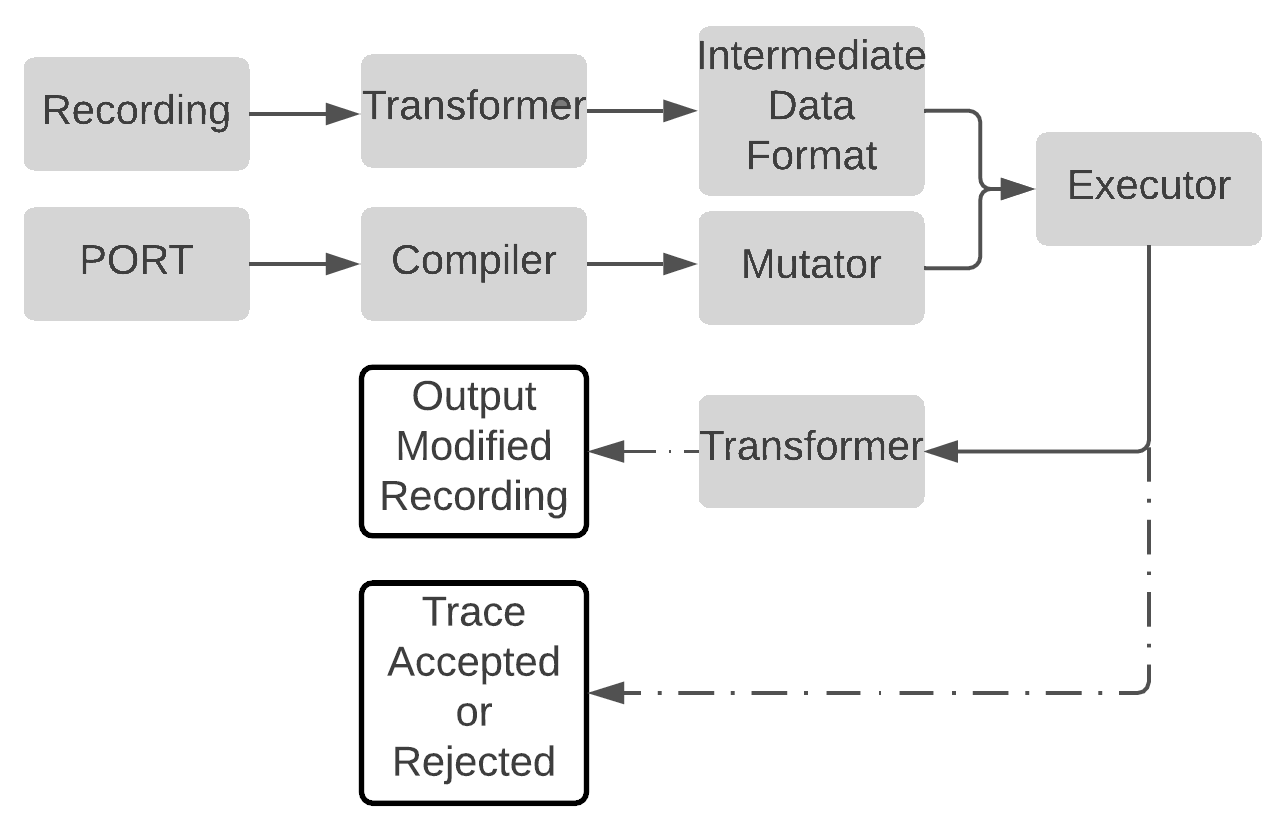
\includegraphics[scale=.08]{images/architecture}
  \caption{The CSLang compiler produces a transducer that operates over a
  generic internal data format that contains the contents of an application
  recording.}
  \label{fig:architecture}
\end{figure}

\subsection{The CSlang Compiler}

The CSlang compiler is responsible for constructing a CSlang transducer
from a CSlang program.  Once constructed, this automaton is serialized to
disk so that it may be stored and reused.
We made the decision to make CSlang a compiled language because
experience has shown that CSlang programs are typically
compiled a few times during construction
and executed many times over many different applications.
By compiling ahead of time we save the performance cost associated with other
approaches like just-in-time compilation or execution via an interpreter.


\subsection{Supporting Many Activity Representations}

In order to take the SEA technique beyond system calls we wanted to make
CSlang flexible enough that it could work with many different sorts of
activity representations.
To achieve this objective we needed to cleanly separate the details of how
an application's activity was recorded from the representation that will be
processed by a CSlang transducer.
Our solution was twofold.  First, we developed an internal data format
(IDF) that
could store the key components, such as parameter and return values,
of application activities like function
calls and system calls.  This format supports primitive string and numeric
values as well as arbitrarily nested structures in the form of records.
These decisions were based on the Linux kernel's system call implementation
which allows system call inputs and outputs in the form of primitive data
values and complex C structures.
If CSlang were going to support system calls, these capabilities would be
necessary and, further, we found that the same capabilities allowed us to
support other activity representations.

The second component is the set of modules, known as transformers, that can
convert an activity stream from its original representation into IDF and
back.  A transformer achieves the former by parsing each activity entry,
extracting the relevant fields, and assembling this information into an IDF
record.  These records are re-assembled into a stream which is input into a
CSlang transducer.  The result of processing this stream undergoes the
reverse.  The output IDF stream is converted by a transformer back into the
original activity representation.  The current version of CSlang ships with
three transformers:
\begin{itemize}
\item{strace via Posix-Omni-Parser}
\item{JSONRPC via Python's json module}
\item{XMLRPC via Python's lxml module}
\end{itemize}


\subsection{Executing a CSlang Program}

Unlike an executable program, a compiled CSlang program is a static entity
that cannot run by itself.  Instead, a component we refer to as the
``CSlang Executor'' is responsible for carrying out the ancillary work
required to analyze an application recording with a CSlang transducer.
These tasks include deserializing a stored transducer from disk, converting
the selected input stream to CSlang's internal data format using an
appropriate transformer, translating the output stream back to the original
activity representation, and reporting whether the input sequence was
accepted or rejected by the transducer. 

%\begin{itemize}
%  \item{Language describing anomalies}
%  \item{Formal model of transducer that can implement anomalies}
%  \item{Tool to compile description into said formal transducer}
%  \item{Format-agnostic intermediate data structure (IDS) over which transducer
%  operates}
%  \item{Translation layer for converting to and from concrete data into IDS}
%\end{itemize}

\subsection{Nuts and Bolts}

